\section{Background}
\label{sec:background}

\subsection{Task-Oriented Dialog System}
The architecture of a task-oriented dialog system
for online shopping guide assistant is illustrated in \figref{fig:dialog-system}.
It consists of three components like any common dialog systems:
natural language understanding (NLU), 
dialog management (DM), 
and natural language generation (NLG).
In addition, the system also interacts with a product search engine
for the purpose of shopping guide. 
\begin{figure}[h]
	\centering
	\epsfig{file=figures/dialog_system.eps, width=1.0\columnwidth}
	\caption{Pipeline framework of task-oriented dialog system for shopping guide assistant.}
	\label{fig:dialog-system}
	\vspace{-10pt}
\end{figure}

In general, NLU contains two modules: 
\textbf{Intent Detection} and \textbf{Slot Filling}.
Intent Detection aims to predict which product category 
a user is going to buy,
such as dress or t-shirt and so on.
This paper focus on optimizing Slot Filling
and we will detailed introduce it in the rest of this paper.

\subsection{Slot Filling}
\label{sec:slot_filling}
A major task in natural language understanding (NLU) is to extract semantic constituents
by using the words of input text to fill in predefined slots in a semantic frame \cite{mesnil2015using},
which is often referred to as slot filling.
Slot filling can also be regarded as assigning
an appropriate semantic label to each word in
the given input text.

In the case of E-commerce shopping, 
there are three Named Entity types including 
\emph{Category}, \emph{Property Key} and \emph{Property Value}.
We show a real example in \tabref{tab:slot-filling-demo}
and follow the popular in/out/begin (IOB) annotation scheme.
In the named entity level,
``连衣裙''\emph{(dress)} is a Category (\textbf{B-CG}/\textbf{I-CG}),
while ``品牌''\emph{(brand)} is labeled as Property Key
(\textbf{B-PK}/\textbf{I-PK}),
which is the name of one product property.
``耐克''\emph{(Nike)} and ``黑色''\emph{(black)} are labeled as Property Value
(\textbf{B-PV}/\textbf{I-PV}) since they are concrete property values.
However, labeling as Property Value is not good enough for NLU.
Thus, in Slot Filling level, 
we further label ``耐克''\emph{(Nike)} as Brand Property (\textbf{B-Brand}/\textbf{I-Brand}), 
and ``黑色''\emph{(black)} as 
Color Property (\textbf{B-Color}/\textbf{I-Color}).
In the meantime, 
other words in the example utterance that carry no semantic meaning are assigned \textbf{O} label.

The above mentioned semantic labels are defined by 
an extern E-commerce Knowledge Base. 
For example, there are 26 semantic labels in the Dress Category,
which describe different properties for a dress such as color and brand.
%so that we classify them as Property Value (\textbf{PV}) type.
Plus \textbf{PK}, \textbf{CG} and \textbf{O},
there are totally 29 (57 in IOB scheme) slot labels (refer to \tabref{tab:slot-labels}).
Compared to the most well-known dialog state tracking challenge (DSTC) dataset,
in which there are only 9 slot labels in DSTC1\footnote{\url{http://research.microsoft.com/en-us/events/dstc/}} for bus booking scenario
and 8 slot labels in DSTC2\footnote{\url{http://camdial.org/~mh521/dstc/}} for restaurant booking scenario,
our dataset has larger amount of slot labels (29 in total).
Therefore, we call our problem as \emph{Large Scaled Slot Filling} problem.

\begin{table}[htbp]
	\caption{Slot labels defined in E-commerce Knowledge Base}
	\label{tab:slot-labels}
	\centering
	\scriptsize
	\begin{tabular}{c|c|c|c}
		\toprule
		Name Entity & PV & PK & CG \\
		\midrule
		Slot Label & \textbf{Color}, \textbf{Brand}, ... & \textbf{PK} & \textbf{CG} \\
		\midrule
		Example Term & \emph{black}, \emph{Nike}, ... & \emph{brand}, \emph{color}, ... & \emph{dress}, \emph{t-shirt}, ... \\
		\bottomrule
	\end{tabular}
	\vspace{-10pt}
\end{table}

Given an utterance containing a sequence of
words $\textbf{w} = (w_1, w_2, ..., w_T)$,
the goal of slot filling
is to find a sequence of slot labels $\hat{\textbf{y}} = (y_1, y_2, ..., y_T)$, 
one for each word in the utterance, such that:
\begin{equation*}
	\hat{\textbf{y}} = \mathop{\arg\max}_{\textbf{y}}P(\textbf{y}|\textbf{w}).
\end{equation*}

\begin{table*}[htbp]
	\caption{A real example of slot filling in online shoping scenario (IOB scheme).}
	\label{tab:slot-filling-demo}
	\centering
	\scriptsize
	\begin{tabular}{c|c|c|c|c|c|c|c|c|c|c|c|c|c}
		\toprule
		\multirow{2}{*}{Utterance} & 我 & 想 & 买 & 耐 & 克 & 品 & 牌 & 的 & 黑 & 色 & 连 & 衣 & 裙 \\
		\cmidrule{2-14}
		& \em{I} & \em{want} & \em{buy} & \multicolumn{2}{c|}{\em{Nike}} & \multicolumn{2}{c|}{\em{brand}} & $\backslash$  & \multicolumn{2}{c|}{\em{black}} & \multicolumn{3}{c}{\em{dress}} \\
		\midrule
		Slot Label & \textbf{O} & \textbf{O} & \textbf{O} & \textbf{B-Brand} & \textbf{I-Brand} & \textbf{B-PK} & \textbf{I-PK} & \textbf{O} & \textbf{B-Color} & \textbf{I-Color} & \textbf{B-CG} & \textbf{I-CG} & \textbf{I-CG} \\
		\midrule
		Named Entity & \textbf{O} & \textbf{O} & \textbf{O} & \textbf{B-PV} & \textbf{I-PV} & \textbf{B-PK} & \textbf{I-PK} & \textbf{O} & \textbf{B-PV} & \textbf{I-PV} & \textbf{B-CG} & \textbf{I-CG} & \textbf{I-CG} \\
		\midrule
		Segment & \textbf{O} & \textbf{O} & \textbf{O} & \textbf{B} & \textbf{I} & \textbf{B} & \textbf{I} & \textbf{O} & \textbf{B} & \textbf{I} & \textbf{B} & \textbf{I} & \textbf{I} \\
		\bottomrule
	\end{tabular}
	\vspace{-10pt}
\end{table*}

\subsection{RNN Sequence Labeling}
\label{sec:rnn_sequence_labeling}
Slot filling is typically treated as a sequence labeling problem. 
Sequential models such as  conditional
random fields \cite{raymond2007generative} and RNN models \cite{yao2014spoken,mesnil2015using} are among
the most popular methods to solve sequence labeling
tasks. 
\figref{fig:model}(a) 
shows the principle architecture of a BiLSTM-CRF mode,
which is the state-of-the-art model for various sequence labeling tasks \cite{huang2015bidirectional,reimers2017optimal}.
BiLSTM-CRF model consists of BiLSTM layer and CRF layer. 

Bidirectional LSTMs enable the
hidden states to capture both historical and future
context information of the words.
Mathematically, the input of this BiLSTM layer
is a sequence of input vectors,
denoted as $\bi{X}=(\bi{x}_1, \bi{x}_2, ..., \bi{x}_T)$.
The output of BiLSTM layer is a sequence of the hidden
states for each input word, denoted
as $\bi{H}=(\bi{h}_1, \bi{h}_2, ..., \bi{h}_T)$.
Each final hidden state is the concatenation of the forward
$\overrightarrow{\bi{h}_i}$ and backward $\overleftarrow{\bi{h}_i}$ hidden states.
We view BiLSTM as a function $\bilstm(\bi{x}_i)$:

\begin{eqnarray*}
	& \overrightarrow{\bi{h}_i} = \lstm(\bi{x}_i, \overrightarrow{\bi{h}_{i-1}}),
	 \overleftarrow{\bi{h}_i} = \lstm(\bi{x}_i, \overleftarrow{\bi{h}_{i+1}}), \\
	& \bilstm(\bi{x}_i) = \bi{h}_i = [\overrightarrow{\bi{h}_i}(\bi{x}_i);\overleftarrow{\bi{h}_i}(\bi{x}_i)].
\end{eqnarray*}
Most of time we use a Stacking BiLSTM fashion to make the model deeper,
%in which higher layer takes the output state $\bi{h}_i$ of the connected lower layer as input.
in which the output $\bi{h}_i^l$ of layer $l$ becomes the input of layer $l+1$,
e.g. $\bi{h}_i^{l+1}=\bilstm^{l+1}(\bi{h}_i^l)$.

It is always beneficial to consider the correlations
between the current label and neighboring
labels since there are many syntactical constraints
in natural language sentences. For example,
\textbf{I-Brand} will never follow a \textbf{B-Color}. 
If we simply feed the above mentioned hidden states
independently to a Softmax layer to predict the labels\cite{hakanni-tur2016multidomain},
such constraints are more likely
to be broken. Linear-chain Conditional Random
Field (CRF) \cite{lafferty2001conditional} 
is the most popular way to control the structure
prediction and its basic idea is to use a series
of potential function to approximate the conditional
probability of the output label sequence
given the input word sequence.

Formally, we take the above sequence of hidden
states $\bi{H} = (\bi{h}_1, \bi{h}_2, ..., \bi{h}_T)$
as input to the CRF layer,
and its output is final prediction label sequence
$\bi{y} = (y_1, y_2, ..., y_T)$,
where $y_i$ is in the set of pre-defined target labels.
We denote $\mathcal{Y}(\bi{H})$ as the set of all possible label sequences.
Then we derive the conditional probability of the output sequence,
given the input hidden state sequence is:
$$
p(\bi{y}|\bi{H};\bi{W}, \bi{b})=\frac{\prod_{i=1}^{T}\varphi(y_{i-1},y_i,\bi{H})}
{\sum_{\bi{y}'\in\mathcal{y}(\bi{H})}\prod_{i=1}^{T}\varphi(y'_{i-1},y'_i,\bi{H})},
$$
where $\varphi(y',y,\bi{H})=\exp(\bi{W}_{y',y}^{T}\bi{H}+\bi{b}_{y',y})$ are potential functions and $\bi{W}_{y',y}^{T}$ and $\bi{b}_{y',y}$ are weight vector and bias of label pair $(y', y)$.
To train the CRF layer, we use the classic maximum
conditional likelihood estimation and gradient ascent method to train our model.
For a training dataset $\{(\bi{H}_{(i)}, \bi{y}_{(i)})\}$, 
the final log-likelihood is:
$$
L(\bi{W},\bi{b}) = \sum_{i}\log p(\bi{y}_{(i)}|\bi{H}_{(i)};\bi{W},\bi{b}).
$$
Finally, the Viterbi algorithm is adopted
to decode the optimal output sequence $\bi{y}^{*}$:
$$
\bi{y}^{*}=\mathop{\arg\max}_{\bi{y}\in\mathcal{Y}(\bi{H})}p(\bi{y}|\bi{H};\bi{W},\bi{b}).
$$